\documentclass[12pt]{article}\usepackage[]{graphicx}\usepackage[]{xcolor}
% maxwidth is the original width if it is less than linewidth
% otherwise use linewidth (to make sure the graphics do not exceed the margin)
\makeatletter
\def\maxwidth{ %
  \ifdim\Gin@nat@width>\linewidth
    \linewidth
  \else
    \Gin@nat@width
  \fi
}
\makeatother

\definecolor{fgcolor}{rgb}{0.345, 0.345, 0.345}
\newcommand{\hlnum}[1]{\textcolor[rgb]{0.686,0.059,0.569}{#1}}%
\newcommand{\hlstr}[1]{\textcolor[rgb]{0.192,0.494,0.8}{#1}}%
\newcommand{\hlcom}[1]{\textcolor[rgb]{0.678,0.584,0.686}{\textit{#1}}}%
\newcommand{\hlopt}[1]{\textcolor[rgb]{0,0,0}{#1}}%
\newcommand{\hlstd}[1]{\textcolor[rgb]{0.345,0.345,0.345}{#1}}%
\newcommand{\hlkwa}[1]{\textcolor[rgb]{0.161,0.373,0.58}{\textbf{#1}}}%
\newcommand{\hlkwb}[1]{\textcolor[rgb]{0.69,0.353,0.396}{#1}}%
\newcommand{\hlkwc}[1]{\textcolor[rgb]{0.333,0.667,0.333}{#1}}%
\newcommand{\hlkwd}[1]{\textcolor[rgb]{0.737,0.353,0.396}{\textbf{#1}}}%
\let\hlipl\hlkwb

\usepackage{framed}
\makeatletter
\newenvironment{kframe}{%
 \def\at@end@of@kframe{}%
 \ifinner\ifhmode%
  \def\at@end@of@kframe{\end{minipage}}%
  \begin{minipage}{\columnwidth}%
 \fi\fi%
 \def\FrameCommand##1{\hskip\@totalleftmargin \hskip-\fboxsep
 \colorbox{shadecolor}{##1}\hskip-\fboxsep
     % There is no \\@totalrightmargin, so:
     \hskip-\linewidth \hskip-\@totalleftmargin \hskip\columnwidth}%
 \MakeFramed {\advance\hsize-\width
   \@totalleftmargin\z@ \linewidth\hsize
   \@setminipage}}%
 {\par\unskip\endMakeFramed%
 \at@end@of@kframe}
\makeatother

\definecolor{shadecolor}{rgb}{.97, .97, .97}
\definecolor{messagecolor}{rgb}{0, 0, 0}
\definecolor{warningcolor}{rgb}{1, 0, 1}
\definecolor{errorcolor}{rgb}{1, 0, 0}
\newenvironment{knitrout}{}{} % an empty environment to be redefined in TeX

\usepackage{alltt}

\usepackage{graphicx}
\usepackage{url}
\usepackage{hyperref}
\usepackage{verbatim}
\usepackage[title,titletoc,toc]{appendix}
\usepackage{wasysym}
\usepackage[margin=1.0in]{geometry}
\usepackage{natbib}
\IfFileExists{upquote.sty}{\usepackage{upquote}}{}
\begin{document}


\begin{titlepage}

\begin{center}
{\large Introduction to R} \\[1.5in]

{\LARGE \bf A Sample Rnw Document for use with RStudio} \\[.4in]
by \\[.4in]
{\bf J\"urgen Symanzik} \\[1in]
{\bf Date:} \today \\[.8in]

UTAH STATE UNIVERSITY \\[.2in]
Logan, UT \\[0.2in]
Fall 2020 \\[0.2in]
\end{center}

\thispagestyle{empty}
\vfill
\end{titlepage}


\newpage 

\pagenumbering{roman}

\tableofcontents


\newpage

\pagenumbering{arabic}

\section{Creating an Rnw File}

R \textbf{R} code can be included in an existing \LaTeX\ document by changing the name of the file from myfilename.tex to myfilename.Rnw and opening the Rnw file in RStudio.  Alternatively, use File $\rightarrow$ New File $\rightarrow$ R Sweave and fill in the template. 

R code can be embedded in your \LaTeX\ document in a very similar way to the way it is done in R Markdown. An R chunk starts with \verb|<<>>=| and  ends with \verb|@|.
Here is an example:

\begin{knitrout}
\definecolor{shadecolor}{rgb}{0.969, 0.969, 0.969}\color{fgcolor}\begin{kframe}
\begin{alltt}
\hlstd{pi}
\end{alltt}
\begin{verbatim}
## [1] 3.141593
\end{verbatim}
\end{kframe}
\end{knitrout}


and another:
\begin{knitrout}
\definecolor{shadecolor}{rgb}{0.969, 0.969, 0.969}\color{fgcolor}\begin{kframe}
\begin{alltt}
\hlstd{x} \hlkwb{<-} \hlkwd{rnorm}\hlstd{(}\hlnum{5}\hlstd{)}
\hlstd{x}
\end{alltt}
\begin{verbatim}
## [1]  1.6196031 -0.8706166 -0.2821132  1.0085708 -0.6077414
\end{verbatim}
\end{kframe}
\end{knitrout}

\begin{knitrout}
\definecolor{shadecolor}{rgb}{0.969, 0.969, 0.969}\color{fgcolor}\begin{kframe}
\begin{alltt}
\hlstd{xbar} \hlkwb{<-} \hlkwd{mean}\hlstd{(x)}
\hlstd{xbar}
\end{alltt}
\begin{verbatim}
## [1] 0.1735406
\end{verbatim}
\end{kframe}
\end{knitrout}

We can put options in the \verb|<<>>| (here \verb|<<echo=FALSE>>|):

\begin{knitrout}
\definecolor{shadecolor}{rgb}{0.969, 0.969, 0.969}\color{fgcolor}\begin{kframe}
\begin{verbatim}
## [1] 0.1735406
\end{verbatim}
\end{kframe}
\end{knitrout}

and we can set options that will last for the rest of the document using \verb|opts_chunk$set()|:

\begin{knitrout}
\definecolor{shadecolor}{rgb}{0.969, 0.969, 0.969}\color{fgcolor}\begin{kframe}
\begin{alltt}
\hlstd{opts_chunk}\hlopt{$}\hlkwd{set}\hlstd{(}\hlkwc{prompt}\hlstd{=}\hlnum{TRUE}\hlstd{)}
\end{alltt}
\end{kframe}
\end{knitrout}

\begin{knitrout}
\definecolor{shadecolor}{rgb}{0.969, 0.969, 0.969}\color{fgcolor}\begin{kframe}
\begin{alltt}
\hlstd{> }\hlstd{xbar} \hlkwb{<-} \hlkwd{mean}\hlstd{(x)}
\hlstd{> }\hlstd{xbar}
\end{alltt}
\end{kframe}
\end{knitrout}

We can draw plots:

\begin{knitrout}
\definecolor{shadecolor}{rgb}{0.969, 0.969, 0.969}\color{fgcolor}\begin{kframe}
\begin{alltt}
\hlstd{> }\hlkwd{qqnorm}\hlstd{(}\hlkwd{rnorm}\hlstd{(}\hlnum{1000}\hlstd{))}
\end{alltt}
\end{kframe}
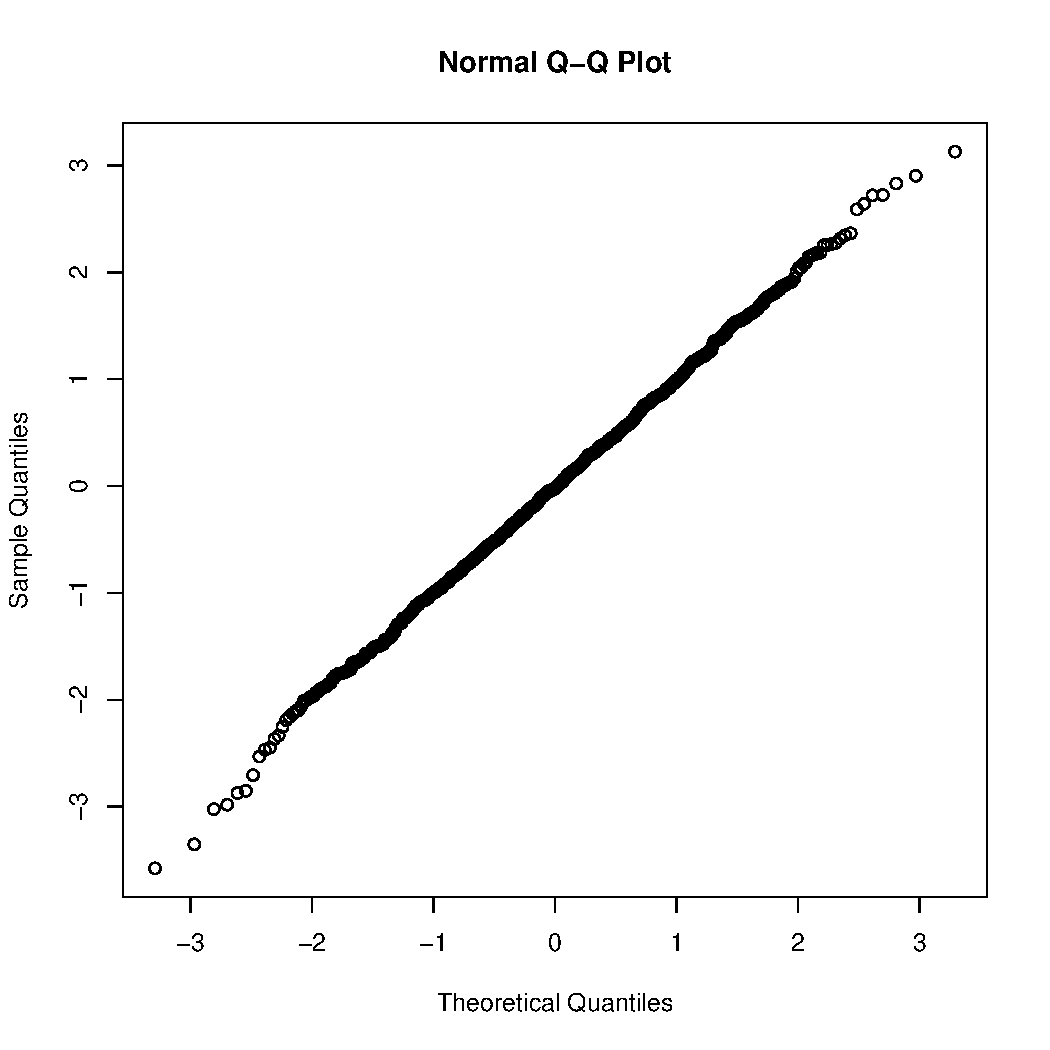
\includegraphics[width=\maxwidth]{figure/unnamed-chunk-8-1} 
\end{knitrout}


\newpage


\section{Multiple Code Chunks}

We can create multiple code chunks and then only evaluate them later on
(look at the Rnw source code to see what happens here):





\begin{knitrout}
\definecolor{shadecolor}{rgb}{0.969, 0.969, 0.969}\color{fgcolor}\begin{kframe}
\begin{alltt}
\hlstd{> }\hlstd{x} \hlkwb{<-} \hlnum{10}
\hlstd{> }\hlstd{y} \hlkwb{<-} \hlnum{20}
\hlstd{> }\hlstd{x} \hlopt{+} \hlstd{y}
\end{alltt}
\begin{verbatim}
## [1] 30
\end{verbatim}
\end{kframe}
\end{knitrout}


\section{Citations and References}

By the way, \LaTeX\ helps you with references and citations via
a bibtex (.bib) file. Once a reference has been entered into such a file,
you can just cite it. Below are some examples:

\begin{itemize}
\item Here a citation ``as noun'':
\textbf{Lamport85} is a main reference for \LaTeX.

\item Here a citation in parentheses:
Several sources for help with knitr exist \textbf{knitr2013}.

\item You can combine multiple references: These references
\textbf{CART,bagging,RF} likely will be used in some of Adele Cutler's courses.
\end{itemize}

Note that the reference list is created automatically! The file ``agsm.bst''
determines the appearance of the references. Most publishers and journals
provide their own bst file so the references will appear immediately
in the proper book or journal style.


%\bibliographystyle{agsm}


%\bibliography{Citations}


\end{document}

